\instructions{ Primarily this is to document the architecture for the stakeholders, to ensure that it meets their goals and concerns and that the proposed architecture is correct, complete and fit for purpose.

  While you should avoid presenting a lot of material available elsewhere, it may also be useful to do some or all of the following in the AD:
  \begin{itemize}
  \item summarise the project context, goals and objectives
  \item confirm scope and exclusions
  \item present an overview of goals and drivers, requirements etc
  \item record important decisions made and their rationale
  \item present alternatives considered and their reasons for rejection
  \item bring together other important information not captured elsewhere
  \end{itemize}
}

\subsection{Scope}
\paragraph{Included}
\begin{itemize}
\item Things for rent
\item Search
\item Requests
\item Billing + Deposits
\item Website
\item Tracking of things
\item Website + Server-stuffs
\end{itemize}

\paragraph{Excluded}
\begin{itemize}
\item Sales
\item Errors + Damage to things
\item Hardware stuffs
\item Verification of transfers
\end{itemize}

\begin{figure}
\centering
    \includegraphics[width=0.7\textwidth]{figures/context_drawing}
    \caption{The context of th system}
    \label{fig:context}
\end{figure}
